

\documentclass[xcolor=table]{beamer}

\mode<presentation> {

% The Beamer class comes with a number of default slide themes
% which change the colors and layouts of slides. Below this is a list
% of all the themes, uncomment each in turn to see what they look like.

%\usetheme{default}
%\usetheme{AnnArbor}
%\usetheme{Antibes}
%\usetheme{Bergen}
%\usetheme{Berkeley}
%\usetheme{Berlin}
%\usetheme{Boadilla}
\usetheme{CambridgeUS}
%\usetheme{Copenhagen}
%\usetheme{Darmstadt}
%\usetheme{Dresden}
%\usetheme{Frankfurt}
%\usetheme{Goettingen}
%\usetheme{Hannover}
%\usetheme{Ilmenau}
%\usetheme{JuanLesPins}
%\usetheme{Luebeck}
%\usetheme{Madrid}
%\usetheme{Malmoe}
%\usetheme{Marburg}
%\usetheme{Montpellier}
%\usetheme{PaloAlto}
%\usetheme{Pittsburgh}
%\usetheme{Rochester}
%\usetheme{Singapore}
%\usetheme{Szeged}
%\usetheme{Warsaw}
\usepackage{pstricks,pst-node,multido}
\usepackage{pstricks,pst-3dplot}
% As well as themes, the Beamer class has a number of color themes
% for any slide theme. Uncomment each of these in turn to see how it
% changes the colors of your current slide theme.

%\usecolortheme{albatross}
%\usecolortheme{beaver}
%\usecolortheme{beetle}
%\usecolortheme{crane}
%\usecolortheme{dolphin}
%\usecolortheme{dove}
%\usecolortheme{fly}
%\usecolortheme{lily}
%\usecolortheme{orchid}
%\usecolortheme{rose}
%\usecolortheme{seagull}
\usecolortheme{seahorse}
%\usecolortheme{whale}
%\usecolortheme{wolverine}

%\setbeamertemplate{footline} % To remove the footer line in all slides uncomment this line
%\setbeamertemplate{footline}[page number] % To replace the footer line in all slides with a simple slide count uncomment this line

%\setbeamertemplate{navigation symbols}{} % To remove the navigation symbols from the bottom of all slides uncomment this line
}

\usepackage[spanish,es-noshorthands]{babel}%correción para evitar extra {
\usepackage[utf8]{inputenc}
\usepackage{graphicx} % Allows including images
\usepackage{booktabs} % Allows the use of \toprule, \midrule and \bottomrule in tables

%----------------------------------------------------------------------------------------
%	TITLE PAGE
%----------------------------------------------------------------------------------------

\title[Programación Orientada a Objetos con C++]{Programación Orientada a Objetos con C++: Conceptos Iniciales} % The short title appears at the bottom of every slide, the full title is only on the title page

\author{R\'omulo Walter Condori Bustincio} % Your name
\institute[] % Your institution as it will appear on the bottom of every slide, may be shorthand to save space
{
UNSA, Arequipa, Per\'u \\ % Your institution for the title page
\medskip
\textit{ rcondorib@unsa.edu.pe} % Your email address
}
\date{\today} % Date, can be changed to a custom date

\begin{document}

\begin{frame}
\titlepage % Print the title page as the first slide
\end{frame}

\begin{frame}
\frametitle{Sumario} % Table of contents slide, comment this block out to remove it
\tableofcontents % Throughout your presentation, if you choose to use \section{} and \subsection{} commands, these will automatically be printed on this slide as an overview of your presentation
\end{frame}

%----------------------------------------------------------------------------------------
%	PRESENTATION SLIDES
%----------------------------------------------------------------------------------------
%------------------------------------------
%------------------------------------------------
\section{Introducci\'on} 
\begin{frame}
\frametitle{Introducci\'on}
C fu\'e implementado en 1972 por Dennis Ritchie en los Laboratorios Bell. Inicialmente se hizo conocido como el lenguaje de desarrollo del sistema operativo UNIX. Hoy en día, la mayor parte del código para sistemas operativos de uso general está escrito en C o C ++. C ++ evolucionó a partir de C, que está disponible para la mayoría de las computadoras y es independiente del hardware. Con un diseño cuidadoso, es posible escribir programas en C que sean portátiles a la mayoría de las computadoras.
\end{frame}

\begin{frame}
\frametitle{Introducci\'on}    
\begin{figure}
    \centering
    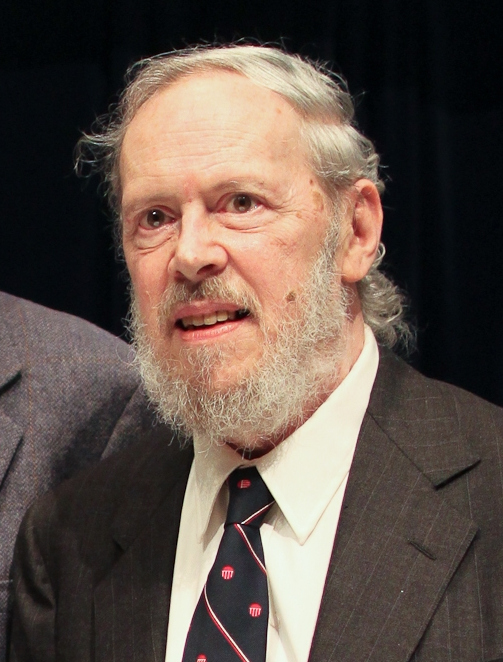
\includegraphics{images/DennisRitchie.jpg}
    \caption{Dennis Ritchie creador de C, fuente: \url{https://es.wikipedia.org/wiki/Dennis_Ritchie}}
    \label{fig:critchie}
\end{figure}
\end{frame}

\begin{frame}
\frametitle{Introducci\'on} 
\begin{figure}
    \centering
    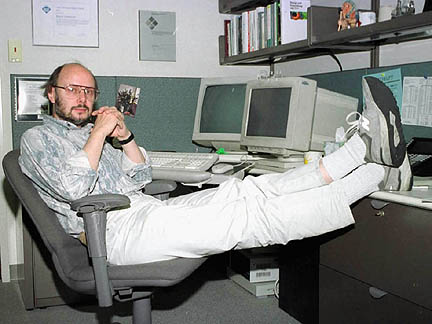
\includegraphics[scale=0.5]{images/BjarneStroustrup.jpg}
    \caption{Bjarne Stroustrup creador de C++ fuente: \url{https://es.wikipedia.org/wiki/Bjarne_Stroustrup}}
    \label{fig:cplusbjarne}
\end{figure}
\end{frame}

\section{Jerarquía de Datos}
\begin{frame}
\frametitle{Jerarquía de Datos}
Los elementos de datos procesados por computadoras forman una jerarquía de datos que se hace más grande y compleja en su estructura a medida que avanzamos desde los elementos de datos más simples (llamados "bits") a los más complejos, como los caracteres y campos. La figura \ref{fig:jeraquia} ilustra una parte de la jerarquía de datos. \cite{deitel}
\end{frame}

\begin{frame}
\frametitle{Jerarquía de Datos}
\begin{figure}
    \centering
    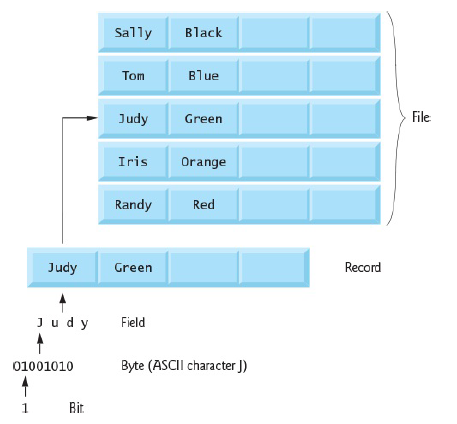
\includegraphics[scale=0.5]{images/dataHierarchy.png}
    \caption{Jerarquía de Datos \cite{deitel} }
    \label{fig:jeraquia}
\end{figure}
\end{frame}
\section{Componentes y Conceptos Básicos}
\begin{frame}
\frametitle{Componentes Básicos}
C ++ es un lenguaje compilado. Para que un programa se ejecute, su texto de origen debe ser procesado por un compilador, que produce archivos objeto (.obj), que se combinan mediante un enlazador(\emph{linker}) que produce un programa ejecutable. Un programa de C ++ generalmente consta de muchos archivos de código fuente (usualmente llamados archivos fuente) \cite{bjarne1}. La figura \ref{fig:compilar} muestra el proceso de compilación.
\end{frame}
\begin{frame}
\frametitle{Componentes y Conceptos Básicos}
\begin{figure}
    \centering
    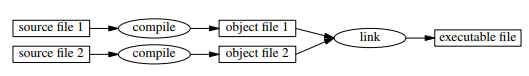
\includegraphics[scale=0.85]{images/compile.png}
    \caption{Proceso de Compilación, Se crea un programa ejecutable para una combinación específica de hardware/sistema; no es portátil, digamos, de una Mac a una PC con Windows. \cite{bjarne1}}
    \label{fig:compilar}
\end{figure}

\end{frame}

\subsection{Estándar C++}
\begin{frame}
\frametitle{Tipos de Entidades en  Estándar ISO-C++}
El estándar ISO C ++ define dos tipos de entidades:
\begin{itemize}
\item Características básicas del lenguaje, como los tipos incorporados (por ejemplo, \textbf{char} y \textbf{int}) y los bucles (por ejemplo, \textbf{for}, \textbf{while}, etc)
\item Componentes de la biblioteca estándar, como contenedores (por ejemplo, \textbf{vector} y \textbf{map}) y operaciones de E/S
(por ejemplo, \textbf{<<}, \textbf{cout})
\end{itemize}
\end{frame}

\subsection{Archivos Fuente y Cabecera}
\begin{frame}
\frametitle{Archivos Fuente y Cabecera}

\end{frame}

\section{Tipos de Datos}
\begin{frame}
\frametitle{Tipos de Datos}

\end{frame}

\subsection{Tipos de Datos Primitivos}
\begin{frame}
\frametitle{Tipos de Datos Primitivos}

\end{frame}

\subsection{Tipos de Datos Abstractos}
\begin{frame}
\frametitle{Tipos de Datos Abstractos}

\end{frame}

\section{Estructuras de Control}
\begin{frame}
\frametitle{Estructuras de Control}    
\end{frame}

\subsection{Estructuras Secuenciales}
\begin{frame}
\frametitle{Estructuras Secuenciales}    
\end{frame}

\subsection{Estructuras Condicionales}
\begin{frame}
\frametitle{Estructuras Condicionales}    
\end{frame}


\subsection{Estructuras Repetitivas}
\begin{frame}
\frametitle{Estructuras Repetitivas}    
\end{frame}


\begin{frame}
\frametitle{Agradecimientos y Preguntas}
\centering
    \Huge{``Muchas Gracias''}
\end{frame}

\begin{frame}
\frametitle{Referencias}
\footnotesize{
\setbeamertemplate{bibliography item}[book]
\begin{thebibliography}{99} % Beamer does not support BibTeX so references must be inserted manually as below

\bibitem[Deitel, 2017]{deitel}
Paul Deitel and Harvey Deitel. 2017. \emph{C++ how to Program (10th ed.)}. Prentice Hall Press, Upper Saddle River, NJ, USA.

\bibitem[Stroustrup, 2013]{bjarne1}
Bjarne Stroustrup. 2013. \emph{The C++ Programming Language (4th ed.)}. Addison-Wesley Professional.

\bibitem[Stroustrup, 2014]{bjarne2}
Bjarne Stroustrup. 2014. \emph{Programming: Principles and Practice Using C++ (2nd Edition) (2nd ed.)}. Addison-Wesley Professional.


\bibitem[Knuth 1984]{p2}
 Donald E. Knuth. 1984. \emph{Literate programming. Comput. J. 27, 2 (May 1984)}, 97-111. DOI=\url{http://dx.doi.org/10.1093/comjnl/27.2.97} 

\end{thebibliography}
}
\end{frame}

%------------------------------------------------
%----------------------------------------------------------------------------------------

\end{document}